\documentclass[11pt]{beamer}

\mode<presentation>
%\usetheme{Frankfurt}
%\usetheme{Boadilla}
\usetheme{Copenhagen}
\setbeamertemplate{navigation symbols}{} 
\setbeamertemplate{caption}[numbered]
\setbeamercolor{block title}{bg=blue}

\usepackage[utf8]{inputenc}
\usepackage{amsmath}
\usepackage{amsfonts}
\usepackage{amssymb}
\usepackage{gensymb}
\usepackage{tikz}

\usetikzlibrary{arrows.meta}

%\author{Alexey L. Cherezov}
\title{Fuel Rod Analysis Program Interface \\(FRAPI)}
%\setbeamercovered{transparent} 
%\setbeamertemplate{navigation symbols}{} 
%\logo{} 
\institute{UNIST Core} 
%\date{} 
%\subject{} 


\tikzset{%
  >={Latex[width=2mm,length=2mm]},
            base/.style = {rectangle, rounded corners, draw=black,
                           minimum width=4cm, minimum height=1cm,
                           text centered, font=\sffamily},
  box0/.style = {base, minimum width=2.5cm, fill=white!15, align=center},
  box1/.style = {base, minimum width=2.5cm, fill=blue!15, align=center},
  box2/.style = {base, minimum width=2.5cm, fill=red!5, align=center},  
  box3/.style = {base, minimum width=2.5cm, fill=green!15, align=center},    
  void/.style = {base, minimum width=2.5cm, fill=white!30, draw=white, align=left},
}


\begin{document}

\titlepage

\begin{frame}{FRAPI Designation}

    \centering{\textbf{The new program interface for FRAPCON and FRAPTRAN}}

 \begin{center}
 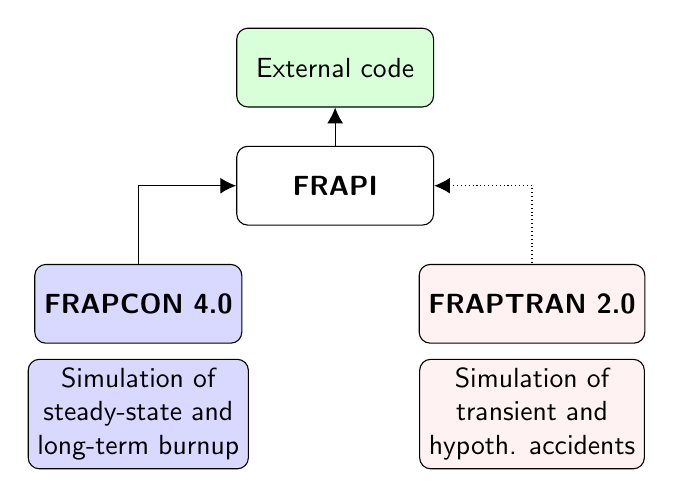
\begin{tikzpicture}[node distance=1.5cm, align=center]

  \node (onFRAPI)    [box0]                                   {\textbf{FRAPI}};
  \node (onCode)     [box3, above of=onFRAPI               ]  {External code};
  \node (onFRAPCON)  [box1, below of=onFRAPI, xshift=-2.5cm]  {\textbf{FRAPCON 4.0}};
  \node (onFRAPTRAN) [box2, below of=onFRAPI, xshift= 2.5cm]  {\textbf{FRAPTRAN 2.0}};  
  \node (on_text_1)  [box1, below of=onFRAPCON, yshift=0.1cm, xshift=0.cm]  {Simulation of \\ steady-state and \\ long-term burnup};
  \node (on_text_2 ) [box2, below of=onFRAPTRAN, yshift=0.1cm, xshift=0cm]  {Simulation of \\ transient and \\ hypoth. accidents};  
  
  \draw[<-]      (onFRAPI) -| (onFRAPCON);
  \draw[<-][densely dotted]      (onFRAPI) -| (onFRAPTRAN);
  \draw[->]      (onFRAPI) -- (onCode);  
  \end{tikzpicture}
  \end{center} 

\end{frame}

\begin{frame}{FRAPI Abilities}

    \centering{\textbf{The FRAPI code:}}

  \begin{block}{}
  1. Provides an access to the most of capability of FRAPCON 
  \textit{\small Except of the decay model ANS-5.1 and the fission gas model ANS-5.4}
  \end{block}

  \begin{block}{}
  2. Exchanges the fuel rod data and algorithm options with an external code ``on the flight", at every time step
  \end{block}

  \begin{block}{}
  3. Dumps the fuel rod data in output file for future restart of a calculation, starting of any chosen time moment
  \end{block}
  
  \vspace{0.5cm}
  \setbeamercolor{block title}{bg=green}
  \begin{block}{}
  \center
  The connection with FRAPTRAN is in progress
  \end{block}
  
\end{frame}

\begin{frame}{FRAPI Testing}

  \scriptsize
   
 \centering{\textbf{Considered 5 benchmarks from NEA Data Bank} \\ 
 \textbf{FRAPI cross-verified with the original FRAPCON version}}

 \begin{center}
 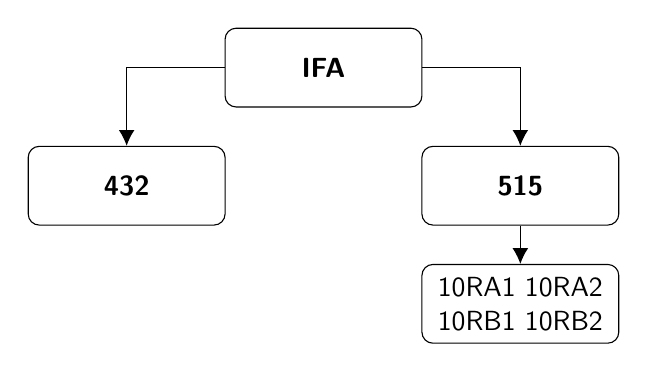
\begin{tikzpicture}[node distance=1.5cm, align=center]

  \node (onIFA)   [box0]                                 {\textbf{IFA}};
  \node (on432)   [box0, below of=onIFA, xshift=-2.5cm]  {\textbf{432}};
  \node (on515)   [box0, below of=onIFA, xshift= 2.5cm]  {\textbf{515}};  
  \node (on515_)  [box0, below of=on515, xshift= 0.0cm]  {10RA1 10RA2 \\ 10RB1 10RB2};    
  
  \draw[->] (onIFA) -| (on432);
  \draw[->] (onIFA) -| (on515);
  \draw[->] (on515) -- (on515_);
  \end{tikzpicture}
  \end{center} 

\end{frame}


\begin{frame}{IFA-432-R3 Benchmark}
  \footnotesize 
  
  \begin{columns}[t]

  \column{.49\textwidth}

  \begin{figure}[h]
    \includegraphics[width=1.\textwidth]{../graphics/IFA-432-r3/average_fuel_burnup}
    \caption{Mechanical gap thickness}
  \end{figure}  

  \column{.49\textwidth}

  \begin{figure}[h]
    \includegraphics[width=1.\textwidth]{../graphics/IFA-432-r3/average_linear_power}    
    \caption{Average linear power}
  \end{figure}  
  
  \end{columns}

\end{frame}


\begin{frame}{IFA-432-R3 Benchmark (continuous)}
  \footnotesize 
  
  \begin{columns}[t]

  \column{.49\textwidth}

  \begin{figure}[h]
    \includegraphics[width=1.\textwidth]{../graphics/IFA-432-r3/centerline_temperature}
    \caption{Centerline fuel temperature, $C$}
  \end{figure}  

  \column{.49\textwidth}

  \begin{figure}[h]
    \includegraphics[width=1.\textwidth]{../graphics/IFA-432-r3/cladding_average_temperature}    
    \caption{Cladding average temperature, $C$}
  \end{figure}  
  
  \end{columns}

\end{frame}

\begin{frame}{IFA-432-R3 Benchmark (continuous)}
  \footnotesize 
  
  \begin{columns}[t]

  \column{.49\textwidth}

  \begin{figure}[h]
    \includegraphics[width=1.\textwidth]{../graphics/IFA-432-r3/cladding_hoop_strain}
    \caption{Cladding hoop strain}
  \end{figure}  

  \column{.49\textwidth}

  \begin{figure}[h]
    \includegraphics[width=1.\textwidth]{../graphics/IFA-432-r3/cladding_hoop_stress}    
    \caption{Cladding hoop stress}
  \end{figure}  
  
  \end{columns}

\end{frame}


\begin{frame}{IFA-432-R3 Benchmark (continuous)}
  \footnotesize 
  
  \begin{columns}[t]

  \column{.49\textwidth}

  \begin{figure}[h]
    \includegraphics[width=1.\textwidth]{../graphics/IFA-432-r3/fission_gas_release}
    \caption{Fission gas release}
  \end{figure}  

  \column{.49\textwidth}

  \begin{figure}[h]
    \includegraphics[width=1.\textwidth]{../graphics/IFA-432-r3/oxide_thickness}    
    \caption{Oxide thickness}
  \end{figure}  
  
  \end{columns}

\end{frame}



\begin{frame}{FRAPI Usage Example}
  \footnotesize
  \texttt{
  \begin{columns}
  \column{0.48\textwidth}
  \begin{block}{}
    {\color{magenta}PROGRAM} MAIN\\
    {\color{magenta}USE} frapi, {\color{magenta}ONLY}: frodtype\\
    {\color{magenta}TYPE} (frodtype) FR\\    
    {\color{gray}!--- Setup mesh size -----}\\
    {\color{magenta}CALL} FR $\%$ MAKE(<arguments>)\\
    {\color{gray}!--- Setup initial state ----}\\    
    {\color{magenta}CALL} FR $\%$ SET({\color{orange}"varname"}, var)\\
    {\color{magenta}CALL} FR $\%$ INIT()\\
    {\color{magenta}CALL} FR $\%$ GET({\color{orange}"varname"}, var)\\
    {\color{gray}!--- Accept initial state ----}\\                
    {\color{magenta}CALL} FR $\%$ ACCEPT()\\    
  \end{block}
  \column{0.48\textwidth}
  \begin{block}{}
    {\color{gray}!--- Burnup loop ---------}\\        
    {\color{magenta}DO} i = 1, N\\
    {\color{gray}!--- Trial time step -----}\\            
    {\hspace{5mm}\color{magenta}CALL} FR $\%$ SET({\color{orange}"varname"}, var)\\
    {\hspace{5mm}\color{magenta}CALL} FR $\%$ NEXT(dtime)\\
    {\hspace{5mm}\color{magenta}CALL} FR $\%$ GET({\color{orange}"varname"}, var)\\
    {\color{gray}!--- Accept time step ----}\\                
    {\hspace{5mm}\color{magenta}CALL} FR $\%$ ACCEPT()\\    
    {\color{gray}!--- Save current state --}\\                
    {\hspace{5mm}\color{magenta}CALL} FR $\%$ SAVE({\color{orange}"filename"})\\    
    {\color{magenta}ENDDO} \\
    {\color{gray}!--- Finilize -------------}\\                    
    {\color{magenta}CALL} FR $\%$ DESTROY()\\            
    {\color{magenta}END PROGRAM}  MAIN
  \end{block}
  \end{columns}
  }
\end{frame}


\begin{frame}{FRAPI Initialization}
  
  \scriptsize
  
  \centering{\textbf{List of ``MAKE"" arguments:}}

  \begin{block}{}
    \begin{itemize}
    \item \texttt{NR} : number of radial segments
    \item \texttt{NA} : number of axial segments
    \item \texttt{NGASR} : number of radial gas release nodes
    \item \texttt{NCE} : number of radial nodes in a cladding of FEA model
    \item \texttt{MECHAN} : cladding mechaniccal model (1: FEA, 2: FRACAS)
    \item \texttt{NGASMOD} : fission gas release model
    \item \texttt{ICM} : cladding type
    \item \texttt{ICOR} : crud model (0 or 1 : constant, 2: time dependent)    
    \item \texttt{IPLANT} : plant type (-2: PWR, -3: BWR, -4: HBWR)
    \item \texttt{IMOX} : fuel type   
    \end{itemize}
  \end{block}
  
\end{frame}


\begin{frame}{FRAPI Initialization (continuous)}
  
  \scriptsize
  
  \centering{\textbf{List of ``MAKE"" arguments:}}

  \begin{block}{}
    \begin{itemize}
    \item \texttt{IGASCAL} : internal pressure calculation for FEA model 
    \item \texttt{ZR2VINTAGE} : zircaloy-2 vintage
    \item \texttt{MOXTYPE} : flag for type of Pu used in MOX
    \item \texttt{IDXGAS} : fill gas type
    \item \texttt{IQ} : axial power shape indicator (0 = user-input, 1 = chopped cosine)
    \item \texttt{IVARDM} : option to specify variable axial node length (1 is on, 0 is off)
    \item \texttt{IFFIXEDCOOLT} : specify user-supplied coolant temperatures (0: off, 1: on)
    \item \texttt{IFFIXEDCOOLP} : Specify use user-supplied coolant pressures (0: off, 1: on)
    \item \texttt{IFFIXEDSURF} : Specify to use fixed cladding surface temperatures
    \item \texttt{VERBOSE} : Print the output data in terminal   
    \end{itemize}
  \end{block}
  
\end{frame}


\end{document}


%%%%%%%%%%%%%%%%%%%%%%%%%%%%%%%%%%%%%%%%%%%%%%%%%%%%%%%%%%%%%%%%%%%%%%%%555




\begin{frame}{FRAPCON}
\scriptsize

  \begin{block}{FRAPCON-4.0}
   Steady-state Long-term Burnup
   \begin{itemize}
   \item Thermal response
   \item Mechanical response
   \item Fission gas release
   \item Waterside corrosion
   \item Hydrogen pickup
   \end{itemize}
  \end{block}

\end{frame}

\begin{frame}{FRAPTRAN}
\scriptsize

  \begin{block}{FRAPTRAN-2.0}
   Transient and Hypotherical Accidents
   \begin{itemize}
   \item Thermal response
   \item Mechanical response
   \item High-temperature corrosion
   \item PCMI cladding failure model
   \item Cladding balooning failure model
   \end{itemize}
  \end{block}

\end{frame}

\begin{frame}{FRAPCON Coupling Interface}

\footnotesize

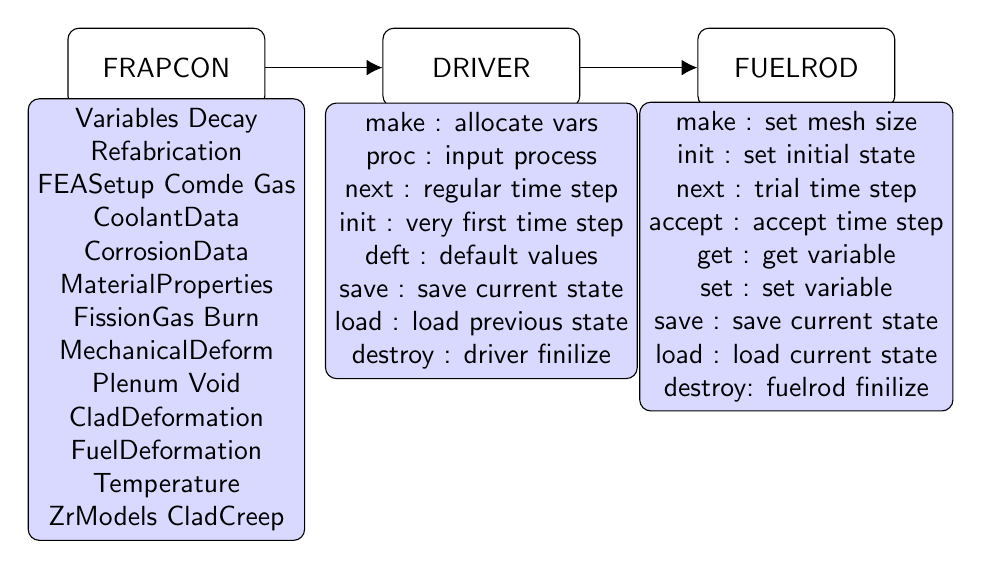
\begin{tikzpicture}[node distance=1.5cm, every node/.style={fill=white, font=\sffamily}, align=center]

  \node (onFrapcon)    [box0]                                      {FRAPCON};
  \node (onDriver)     [box0, right of=onFrapcon,  xshift= 2.5cm]  {DRIVER};
  \node (onFuelrod)    [box0, right of=onDriver,   xshift= 2.5cm]  {FUELROD};  
  \node (onFrapcon_)   [box1, below of=onFrapcon,  yshift=-1.7cm]  
  {Variables Decay \\ 
   Refabrication \\
   FEASetup Comde Gas \\
   CoolantData \\
   CorrosionData \\
   MaterialProperties \\
   FissionGas Burn\\
   MechanicalDeform \\
   Plenum Void \\
   CladDeformation \\
   FuelDeformation \\
   Temperature \\
   ZrModels CladCreep};
  \node (onDriver_)    [box1, below of=onDriver,   yshift=-0.7cm]  
  {make : allocate vars \\ 
   proc : input process \\ 
   next : regular time step \\ 
   init : very first time step \\ 
   deft : default values \\ 
   save : save current state \\ 
   load : load previous state \\
   destroy : driver finilize};
  \node (onFuelrod_)   [box1, below of=onFuelrod,  yshift=-0.9cm]  
  {make   : set mesh size \\ 
   init   : set initial state \\ 
   next   : trial time step \\ 
   accept : accept time step \\ 
   get    : get variable \\ 
   set    : set variable \\ 
   save   : save current state \\ 
   load   : load current state \\
   destroy: fuelrod finilize };  
  
  \draw[->]      (onFrapcon) -- (onDriver);
  \draw[->]      (onDriver)  -- (onFuelrod);
  \end{tikzpicture}
  
\end{frame}




\begin{frame}{Features of the DRIVER module}
  \footnotesize

  \begin{block}{Time integration:}
  \begin{itemize}
    \item Restarting of the input data from the previous time step
    \item Reading and adjustment of variables amid two time steps
  \end{itemize}
  \end{block}

  \begin{block}{Switched off models:}
  \begin{itemize}
    \item Decay model ANS-5.1 (2005)
    \item Fission gas response model ANS-5.4 (1952)
  \end{itemize}
  \end{block}

\end{frame}


\begin{frame}{Initialization and running}
  
  \footnotesize

  \begin{block}{\texttt{make(m,n,dx,rf,rg,rc,pitch,den,enrch)}}
    \begin{itemize}
    \item \texttt{m, n} : number of radial and axial segments
    \item \texttt{dx} : axial node thickness, cm
    \item \texttt{rfuel, rgap, rclad} : radius of fuel, gap and cladding, cm
    \item \texttt{pitch} : fuel rod pitch, cm
    \item \texttt{den} : as-fabricated apparent fuel density, $\%$
    \item \texttt{enrch} : initial fuel enrichment, $\%$
    \end{itemize}
  \end{block}

  \begin{block}{\texttt{init()}}
  Make very first time step ($10^{-5}$ day) which is needed for stabilization of the time-integration scheme and initialization of the variables
  \end{block}
  
  \begin{columns}

  \column{0.48\textwidth}
  \begin{block}{\texttt{next(dtime)}}
    Performs the trial time step
    \begin{itemize}
    \item \texttt{dtime} : time step, $day$
    \end{itemize}
  \end{block}
  
  \column{0.48\textwidth}
  \begin{block}{\texttt{accept()}}
  If the routine is not called, the last time step would be rejected
  \end{block}

  \end{columns}
  
\end{frame}



\begin{frame}{Running calculations: Settings of parameters}
  
  \footnotesize

  \begin{block}{Set variables : \texttt{set(key, value)}}
    \begin{itemize}
    \item \texttt{key} : name of the variable
    \item \texttt{value} : value of the variable    
    \end{itemize}
  \end{block}

  \begin{block}{List of the available parameters}
    \begin{itemize}
    \item linear power distribution, $\frac{W}{cm}$
    \item coolant temperature distribution, $\degree C$
    \item coolant pressure distribution, $MPa$
    \item coolant mass flux, $\frac{kg}{s \cdot m^2}$
    \end{itemize}
  \end{block}

\end{frame}


\begin{frame}{Running Calculations: Output Data}
  
  \footnotesize

  \begin{block}{Get variables: \texttt{get(key, value)}}
    \begin{itemize}
    \item \texttt{key} : name of the variable
    \item \texttt{value} : value of the variable    
    \end{itemize}
  \end{block}
  
  \begin{columns}
  \column{0.49\textwidth}
  \begin{block}{List of the available parameters}
    \begin{itemize}
    \item axial fuel temperature, $\degree C$
    \item bulk coolant temperature, $\degree C$
    \item gap conductance, $\frac{W}{m^2 \cdot K}$
    \item thermal gap thickness, $\mu m$
    \item mechanical gap thickness, $\mu m$
    \end{itemize}
  \end{block}

  \column{0.49\textwidth}  
  \begin{block}{}
    \begin{itemize}
    \item gap pressure, $MPa$
    \item cladding hoop strain, $\%$
    \item cladding hoop stress, $MPa$
    \item cladding axial stress, $MPa$
    \item cladding radial stress, $MPa$
    \item cladding radial stress, $MPa$
    \item axial mesh, $cm$
    \end{itemize}
  \end{block}

  \end{columns}

\end{frame}


\begin{frame}{Test Example}
  
  \footnotesize

  \begin{block}{Fuel rod}
    \begin{itemize}
    \item Uranium fuel rod with the initial enrichment $x=3.42\%$    
    \item Fuel pellet diameter $d=8.26 mm$, length $h=9.8298 mm$
    \item Fuel stack height $H=3.8333 m$, plenum length $L=16.1 cm$
    \end{itemize}
  \end{block}

  \begin{block}{Initial conditions}
    \begin{itemize}
    \item Average linear heat rating is 14.6 $kW/m$
    \item Coolant inlet temperature is 569 $K$
    \item Coolant mass flux is 3857 $\frac{kg}{s \cdot m^2}$
    \end{itemize}
  \end{block}

  \begin{block}{Transient simulation}
    \begin{itemize}
    \item Transient during 40 days with the time step 5 days
    \item Input parameters are changed: $C(t) = C_0 Sin(\pi t/T)$, where $T=20$ days
    \end{itemize}
  \end{block}

\end{frame}



\begin{frame}{Input parameters}
  \footnotesize 
  
  \begin{columns}[t]

  \column{.49\textwidth}

  \begin{figure}[h]
    \includegraphics[width=1.\textwidth]{figs/axial_fuel_temperature}
    \caption{Axial fuel temperature}
    \label{fig:tfuel}
  \end{figure}  

  \column{.49\textwidth}

  \begin{figure}[h]
    \includegraphics[width=1.\textwidth]{figs/bulk_coolant_temperature}    
    \caption{Bulk coolant temperature}
    \label{fig:tcool}
  \end{figure}  
  
  \end{columns}

\end{frame}



\begin{frame}{Output parameters (1)}
  \footnotesize 
  
  \begin{columns}[t]

  \column{.49\textwidth}

  \begin{figure}[h]
    \includegraphics[width=1.\textwidth]{figs/total_gap_conductance}
    \caption{Total gap conductance}
    \label{fig:conduct}    
  \end{figure}  

  \column{.49\textwidth}

  \begin{figure}[h]
    \includegraphics[width=1.\textwidth]{figs/oxide_thickness}    
    \caption{Oxide thickness}
    \label{fig:oxide}
  \end{figure}  
  
  \end{columns}

\end{frame}


\begin{frame}{Output parameters (2)}
  \footnotesize 
  
  \begin{columns}[t]

  \column{.49\textwidth}

  \begin{figure}[h]
    \includegraphics[width=1.\textwidth]{figs/mechanical_gap_thickness}
    \caption{Mechanical gap thickness}
  \end{figure}  

  \column{.49\textwidth}

  \begin{figure}[h]
    \includegraphics[width=1.\textwidth]{figs/gap_pressure}    
    \caption{Gap pressure}
  \end{figure}  
  
  \end{columns}

\end{frame}

\begin{frame}{Output parameters (3)}
  \footnotesize 
  
  \begin{columns}[t]

  \column{.49\textwidth}

  \begin{figure}[h]
    \includegraphics[width=1.\textwidth]{figs/cladding_hoop_strain}
    \caption{Cladding hoop strain}
  \end{figure}  

  \column{.49\textwidth}

  \begin{figure}[h]
    \includegraphics[width=1.\textwidth]{figs/cladding_axial_stress}    
    \caption{Cladding axial stress}
  \end{figure}  
  
  \end{columns}

\end{frame}


\begin{frame}{Conclusion}
  \footnotesize 

  \begin{block}{Have done}
  \begin{itemize}
  \item DRIVER module for FRAPCON which includes the \textbf{next} routine for the step-by-step integration of the fuel rod burnup transient problem
  \item FPN4RASTK module for coupling with the RAST-K code
  \end{itemize}
  \end{block}
  
  \begin{block}{Future work}
  \begin{itemize}
  \item Fix the difference in oxide thickness and cladding hoop strain
  \item Run the FPN4RASTK module along with the RAST-K code
  \item Check other FRAPCON's physical models and capabilities
  \item Write the documentation for the DRIVER and FPN4RASTK modules 
  \item Verification of FRAPCON with the updated DRIVER module
  \end{itemize}
  \end{block}

\end{frame}

\end{document}

